\documentclass[
    11pt,            % 8-20pt possible
    techreport,        % select between  ``techreport'', ``report'', 
    affiltop,       % switch, put affiliations under authors (instead 
]{art}


% Title
\newcommand{\pubtitle}{Anoma Resource Machine Specification}

\newcommand{\pubauthA}{Yulia Khalniyazova}
\newcommand{\pubaffilA}{a}
% \newcommand{\orcidA}{0000-0001-5477-1503}
\newcommand{\authemailA}{\{yulia, cwgoes\}@heliax.dev}
% \newcommand{\eqcontribA}{}

\newcommand{\pubauthB}{Christopher Goes}
\newcommand{\pubaffilB}{a}
% \newcommand{\orcidB}{0000-0001-0000-0000}
\newcommand{\authemailB}{cwgoes@heliax.dev}
% \newcommand{\eqcontribB}{}

% \newcommand{\pubauthC}{Last Author}
% \newcommand{\pubaffilC}{a}
% \newcommand{\orcidC}{0000-0001-5477-1503}
% \newcommand{\authemailC}{mail@someinstitute.com}

% Institutions/Affiliations
\newcommand{\pubaddrA}{Heliax AG}

% Corresponding author mail
\newcommand{\pubemail}{\authemailA}

\newcommand{\pubabstract}{
The article explores the Anoma Resource Machine (ARM) within the Anoma protocol, providing a comprehensive understanding of its role in facilitating state updates based on user preferences. Drawing parallels with the Ethereum Virtual Machine, the ARM introduces a flexible transaction model, diverging from traditional account and UTXO models. Key properties such as atomic state transitions, information flow control, account abstraction, and an intent-centric architecture contribute to the ARM's robustness and versatility. Inspired by the Zcash protocol, the ARM leverages commitment accumulators to ensure transaction privacy. The article outlines essential building blocks, computable components, and requirements for constructing the ARM, highlighting its unique approach to resource-based state management.
}

% Description of the SI file, placed as a footnote
% \newcommand{\pubSI}{Electronic Supplementary Information (ESI) available:
% one PDF file with all referenced supporting information.}

% Any keywords to be displayed under the abstract
\keywords{
Anoma Resource Machine \sep
resource model \sep
virtual machine \sep 
transaction privacy \sep
 
}

% Supplementary space between title/abstract and text, if needed
% \newcommand{\pubVadj}{0pt}

% ! DO NOT REMOVE OR MODIFY !
% Do not modify this file!

\title{\pubtitle}

\newcommand{\dg}{\textsuperscript{\textbf{\dag\textnormal{,}}}}

\ifdef{\pubauthA}{\author[\pubaffilA]{\pubauthA\ifdef{\orcidA}{~\protect\orcid{\orcidA}}{}\ifdef{\eqcontribA}{\dg}{}}}{}
\ifdef{\pubauthB}{\author[\pubaffilB]{\pubauthB\ifdef{\orcidB}{~\protect\orcid{\orcidB}}{}\ifdef{\eqcontribB}{\dg}{}}}{}
\ifdef{\pubauthC}{\author[\pubaffilC]{\pubauthC\ifdef{\orcidC}{~\protect\orcid{\orcidC}}{}\ifdef{\eqcontribC}{\dg}{}}}{}
\ifdef{\pubauthD}{\author[\pubaffilD]{\pubauthD\ifdef{\orcidD}{~\protect\orcid{\orcidD}}{}\ifdef{\eqcontribD}{\dg}{}}}{}
\ifdef{\pubauthE}{\author[\pubaffilE]{\pubauthE\ifdef{\orcidE}{~\protect\orcid{\orcidE}}{}\ifdef{\eqcontribE}{\dg}{}}}{}
\ifdef{\pubauthF}{\author[\pubaffilF]{\pubauthF\ifdef{\orcidF}{~\protect\orcid{\orcidF}}{}\ifdef{\eqcontribF}{\dg}{}}}{}
\ifdef{\pubauthG}{\author[\pubaffilG]{\pubauthG\ifdef{\orcidG}{~\protect\orcid{\orcidG}}{}\ifdef{\eqcontribG}{\dg}{}}}{}
\ifdef{\pubauthH}{\author[\pubaffilH]{\pubauthH\ifdef{\orcidH}{~\protect\orcid{\orcidH}}{}\ifdef{\eqcontribH}{\dg}{}}}{}
\ifdef{\pubauthI}{\author[\pubaffilI]{\pubauthI\ifdef{\orcidI}{~\protect\orcid{\orcidI}}{}\ifdef{\eqcontribI}{\dg}{}}}{}
\ifdef{\pubauthJ}{\author[\pubaffilJ]{\pubauthJ\ifdef{\orcidJ}{~\protect\orcid{\orcidJ}}{}\ifdef{\eqcontribJ}{\dg}{}}}{}
\ifdef{\pubauthK}{\author[\pubaffilK]{\pubauthK\ifdef{\orcidK}{~\protect\orcid{\orcidK}}{}\ifdef{\eqcontribK}{\dg}{}}}{}

\ifdef{\eqcontribA}{\equalcontrib{}}{}
\ifdef{\eqcontribB}{\equalcontrib{}}{}
\ifdef{\eqcontribC}{\equalcontrib{}}{}
\ifdef{\eqcontribD}{\equalcontrib{}}{}
\ifdef{\eqcontribE}{\equalcontrib{}}{}
\ifdef{\eqcontribF}{\equalcontrib{}}{}
\ifdef{\eqcontribG}{\equalcontrib{}}{}
\ifdef{\eqcontribH}{\equalcontrib{}}{}
\ifdef{\eqcontribI}{\equalcontrib{}}{}
\ifdef{\eqcontribJ}{\equalcontrib{}}{}
\ifdef{\eqcontribK}{\equalcontrib{}}{}

\ifdef{\pubaddrA}{\affil[a]{\pubaddrA}}{}
\ifdef{\pubaddrB}{\affil[b]{\pubaddrB}}{}
\ifdef{\pubaddrC}{\affil[c]{\pubaddrC}}{}
\ifdef{\pubaddrD}{\affil[d]{\pubaddrD}}{}
\ifdef{\pubaddrE}{\affil[e]{\pubaddrE}}{}
\ifdef{\pubaddrF}{\affil[f]{\pubaddrF}}{}
\ifdef{\pubaddrG}{\affil[g]{\pubaddrG}}{}
\ifdef{\pubaddrH}{\affil[h]{\pubaddrH}}{}

\contact{\pubemail}

%% Abstract
%% --------

\begin{abstract}
    \pubabstract{}
\end{abstract}

%% Keywords
%% --------

\ifdef{\pubkeywords}{\keywords{\pubkeywords}}{}

%% Adjusting vertical space
%% ------------------------

\ifdef{\pubVadj}{\verticaladjustment{\pubVadj}}{}

% The preprint DOI to be used as an link in the paper
\pubdoi{10.5281/zenodo.10498991}
\history{(Received Nov 10, 2023; Revised Jan 25, 2024 ; Version:  February 21, 2024)}
% MACROS
\newcommand{\N}{\mathbb{N}}

\newcommand{\JuvixCore}{\ensuremath{\mathsf{JuvixCore}}}
\newcommand{\Geb}{\ensuremath{\mathsf{Geb}\,}}
\newcommand{\Juvix}{\ensuremath{\mathsf{Juvix}}}
\newcommand{\VampIR}{\ensuremath{\mathsf{VampIR}}}
\newcommand{\LambdaIR}{\ensuremath{\mathsf{Lambda}}}


\begin{document}

\maketitle

% \iftoggle{SI}{}{\ifdef{\pubSI}{\footnotetext{\pubSI}}{}}

\tableofcontents

\section{Introduction}

In the Anoma protocol, users submit preferences about the system state and the system continuously updates its state based on those preferences. The Anoma Resource Machine (ARM) is the part of the Anoma protocol that defines and enforces the rules for valid state updates that satisfy users' preferences. The new proposed state is then agreed on by the consensus participants. In that sense the role of the Anoma Resource Machine in the Anoma protocol is similar to the role of the Ethereum Virtual Machine in the Ethereum protocol.

The atomic unit of the ARM state is called a \textbf{resource}. Resources are immutable, they can be created once and consumed once, which indicates the system state change. The resources that were created but not consumed yet make the current state of the system.

The ARM transaction model is neither the account nor UTXO model. Unlike the Bitcoin UTXO model, which sees UTXOs as currency units and is limited in expressivity, the resource model is generalised and provides flexibility — resource logics can be defined in a way to construct applications that operate in either transaction model (or both). 
For example, a token operating in the account model would be represented by a single resource containing a map $user: balance$ (unlike the UTXO model, where the token would be represented by a collection of resources of the token type, each of which would correspond to a portion of the token total supply and belong to some user owning this portion). Only one resource of that kind can exist at a time. When a user wants to perform a transfer, they consume the old balance table resource and produce a new balance table resource.

The Anoma Resource Machine has the following properties:
\begin{itemize}
    \item \textit{Atomic state transitions of unspecified complexity} — the number of resources created and consumed in every atomic state transition is not limited by the system.
    \item \textit{Information flow control} — the parties involved in a transaction can decide how much of the information about their state to reveal and to whom. From the resource machine perspective, these states are treated equally (e.g., there is no difference between transparent and shielded resources), but the amount of information revealed about the states differs. It is realised with the help of \textit{shielded execution}, in which the state transition is only visible to the parties involved.
    \item \textit{Account abstraction} — each resource is controlled by a \textit{resource logic} — a custom predicate that encodes constraints on valid state transitions for that kind of resource and determines if a resource can be created or consumed. A valid state transition requires a resource logic proof for every resource created or consumed in the proposed state transition.
    \item \textit{Intent-centric architecture} — the ARM provides means to express intents and ensures their correct and complete fulfilment and settlement.
\end{itemize} 

The design of the Anoma Resource Machine was significantly inspired by the Zcash protocol (\cite{orchard}).

The rest of the document contains the definitions of the ARM building blocks and the necessary and sufficient requirements to build the Anoma Resource Machine. % well, they should be

\section{Preliminaries}

\subsection{Notation}

For a function $h$, we denote the output finite field of $h$ as $\mathbb{F}_h$. If a function $h$ is used to derive a component $x$, we refer to the function as $h_x$, and the corresponding to $h$ finite field is denoted as $\mathbb{F}_{h_x}$, or, for simplicity, $\mathbb{F}_x$.

%We say $xs$ ("$x$-set") to refer to a set of objects of the same type as $x$.

% Future:
% - specify H properties and stop calling it a hash function
% - we might want to also specify other sub-types of functions, e.g., commitments of certain types, PRFs, etc


\section{Resource}
A \textit{resource} is a composite structure $R = (l, label, q, v, eph, nonce, npk, rseed): Resource$ where:
\begin{itemize}
    \item $Resource = \mathbb{F}_{l} \times \mathbb{F}_{label} \times \mathbb{F}_Q \times \mathbb{F}_{v} \times \mathbb{F}_b \times \mathbb{F}_{nonce} \times  \mathbb{F}_{npk} \times \mathbb{F}_{rseed}$ 
    \item $l: \mathbb{F}_{l}$ is a succinct representation of the predicate associated with the resource (resource logic)
    \item $label: \mathbb{F}_{label}$ specifies the fungibility domain for the resource. Resources within the same fungibility domain are seen as equivalent kinds of different quantities. Resources from different fungibility domains are seen and treated as distinct asset kinds. This distinction comes into play in the balance check described later.
    \item $q: \mathbb{F}_Q$ is an number representing the quantity of the resource
    \item $v: \mathbb{F}_{v}$ is the fungible data of the resource. It contains extra information but does not affect the resource's fungibility
    \item $eph: \mathbb{F}_b$ is a flag that reflects the resource's ephemerality. Ephemeral resources do not get checked for existence when being consumed
    \item $nonce: \mathbb{F}_{nonce}$ guarantees the uniqueness of the resource computable components
    \item $npk: \mathbb{F}_{npk}$ is a nullifier public key. Corresponds to the nullifier key $nk$ used to derive the resource nullifier (nullifiers are further described in \ref{nf})
    \item $rseed: \mathbb{F}_{rseed}$: randomness seed used to derive whatever randomness needed
\end{itemize}

To distinguish between the resource data structure consisting of the resource components and a resource as a unit of state identified by just one (or some) of the resource computed fields, we sometimes refer to the former as a resource plaintext.

\subsection{Computable Components}

Resource computable components are the components that are derivable from the resource components, other computed components, and possibly some secret data by applying a function from class $H$.

\subsubsection{Resource Commitment}

Information flow control property implies working with flexible privacy requirements, varying from transparent contexts, where almost everything is publicly known, to contexts with stronger privacy guarantees, where as little information as possible is revealed.

From the resource model perspective, stronger privacy guarantees require operating on resources that are not publicly known in a publicly verifiable way. Therefore, proving the resource's existence has to be done without revealing the resource's plaintext.

One way to achieve this would be to publish a \textbf{commitment} to the resource plaintext. For a resource $r$, the resource commitment is computed as $r.cm = h_{cm}(r)$. Resource commitment has binding and hiding properties, meaning that the commitment is tied to the created resource but does not reveal information about the resource beyond the fact of creation. From the moment the resource is created, and until the moment it is consumed, the resource is a part of the system's state

\begin{remark}
    The resource commitment is also used as the resource's address $r.addr$ in the content-addressed storage.
\end{remark}

All resource commitments are stored in an append-only data structure called a \textbf{commitment accumulator} $CMacc$. Every time a resource is created, its commitment is added to the commitment accumulator. The resource commitment accumulator $CMacc$ is external to the resource machine, but the resource machine can read from it. A commitment accumulator is a cryptographic accumulator (\cite{DBLP:journals/corr/abs-2103-04330}) that allows to prove membership for elements accumulated in it, provided a witness and the accumulated value.

Each time a commitment is added to the $CMacc$, the accumulator and all witnesses of the already accumulated commitments are updated.
For a commitment that existed in the accumulator before a new one was added, both the old witness and the new witness (with the corresponding accumulated value parameter) can be used to prove membership. However, the older the witness (and, consequently, the accumulator) that is used in the proof, the more information about the resource it reveals (the resource had to exist before it was consumed, and an older accumulator gives more concrete boundaries on the resource's creation time). For that reason, it is recommended to use fresher parameters when proving membership.

The commitment accumulator must support the following functionality:
\begin{itemize}
    \item $WRITE(cm)$ adds an element to the accumulator, returning the witness used to prove membership. 
    \item $WITNESS(cm)$ for a given element, returns the witness used to prove membership if the element is present, otherwise returns nothing.
    \item $VERIFY(cm, w, acc)$ verifies the membership proof for an element $cm$ with a membership witness $w$ in the accumulator $acc$.
    \item $ACC()$ returns the accumulator.
\end{itemize}

% Instantiation details
Currently, the commitment accumulator is assumed to be a Merkle tree $CMtree$ of depth $depth_{CMtree}$, where the leaves contain the resource commitments and the intermediate nodes' values are computed using a hash function $h_{CMtree}$. 

\begin{remark}
    The hash function $h_{CMtree}$ used to compute the nodes of the $CMtree$ Merkle tree is not necessarily the same as the function used to compute commitments stored in the tree $h_{cm}$.
\end{remark}

For a Merkle tree, the witness is the path to the resource commitment, and the tree root represents the accumulated value. To support the systems with stronger privacy requirements, the witness for such a proof must be a private input (\ref{public-private-inputs}) when proving membership.

\subsubsection{Resource Nullifier}\label{nf}

A resource nullifier is a computed field, the publishing of which consumes an existing resource. For a resource $r$, the nullifier is computed from the resource's plaintext and a key called a nullifier key: $r.nf = h_{nf}(nk, r)$. A resource can be consumed only once. Nullifiers of consumed resources are stored in a public add-only structure called the resource nullifier set ($NFset$). This structure is external to the resource machine, but the resource machine can read from it.

%TODO: move it somewhere else?
Every time a resource is consumed, it has to be checked that the resource existed before (the resource's commitment is in the $CMtree$) and has not been consumed yet (the resource's nullifier is not in the $NFset$).

The nullifier set must support the following functionality:
\begin{itemize}
    \item $WRITE(nf)$ adds an element to the nullifier set. 
    \item $EXISTS(nf)$ checks if the element is present in the set, returning a boolean

\end{itemize}
\subsubsection{Resource Kind}
For a resource $r$, its kind is computed as $r.kind = h_{kind}(r.l, r.label)$.

\subsubsection{Resource Delta}\label{delta-resource}
Resource deltas are used to reason about the total quantities of different kinds of resources in transactions. For a resource $r$, its delta is computed as $r.\Delta = h_{\Delta}(r.kind, r.q)$.

\begin{remark}
    The function used to derive $r.\Delta$ must have the following properties:
    \begin{itemize}
    \item For resources of the same kind $kind$, $h_{\Delta}$ should be \textit{additively homomorphic}:
$r_1.\Delta + r_2.\Delta = h_{\Delta}(kind, r_1.q + r_2.q)$
    \item For resources of different kinds, $h_\Delta$ has to be \textit{kind-distinct}: if there exists $kind$ and $q$ s.t. $h_\Delta(r_1.kind, r_1.q) + h_\Delta(r_2.kind, r_2.q) = h_\Delta(kind, q)$, it is computationally infeasible to compute $kind$ and $q$.
\end{itemize}

An example of a function that satisfies these properties is the Pedersen commitment scheme: it is additively homomorphic, and its kind-distinctness property comes from the discrete logarithm assumption.
\end{remark}

\section{Proving system}

A proving system allows proving statements about resources. Depending on the security requirements, a proving system might be instantiated, for example, by a signature scheme, a zk-SNARK, or a trivial transparent system where the properties are proven by openly verifying the properties of published data.

\label{public-private-inputs}
To support the intended spectrum of privacy requirements, varying from the strongest (where the relationship between the published parameters does not allow an observer to infer any kind of meaningful information about the state transition) to the weakest, where no privacy is required, we divide the proving system inputs into public (instance) and private (witness). The inputs that could potentially reveal the connection between components or other kinds of sensitive information are usually considered private, and the components that have to be and can be safely published regardless of the privacy guarantees of the system would be public inputs. Note that in the context of a fully public system, this distinction is not meaningful because all inputs are public in such a system.

We define a set of structures required to define a proving system $PS$ as follows:
\begin{itemize}
    \item Proof $\pi: PS.Proof$
    \item Instance $x: PS.Instance$ is the public input used to produce a proof.
    \item Witness $w: PS.Witness$ is the private input used to produce a proof.
    \item Proving key $pk: PS.ProvingKey$ contains the secret data required to produce a proof for a pair $(x, w)$. 
    \item Verifying key $vk: PS.VerifyingKey$ contains the data required, along with the witness $x$, to verify a proof $\pi$.
\end{itemize}

A \textbf{proof record} carries the components required to verify a proof. It is defined as a composite structure $PR = (\pi, x, vk): ProofRecord$, where:
\begin{itemize}
    \item $ProofRecord = PS.VerifyingKey \times PS.Instance \times PS.Proof$
    \item $vk: PS.VerifyingKey$
    \item $x: PS.Instance$
    \item $\pi: PS.Proof$ is the proof of the desired statement.
\end{itemize}

A proving system $PS$ consists of a pair of algorithms, $(Prove, Verify)$:

\begin{itemize}
    \item $Prove(pk, x, w): PS.ProvingKey \times PS.Instance \times PS.Witness \rightarrow PS.Proof$
    \item $Verify(pr): PS.ProofRecord \rightarrow \mathbb{F}_b$
\end{itemize}

A proving system used to produce ARM proofs should have the following properties (as defined in \cite{thaler}):
\begin{itemize}
    \item \textit{Completeness}. This property states that any true statement should have a convincing proof of its validity.
    \item \textit{Soundness}. This property states that no false statement should have a convincing proof.
    \item Proving systems used to provide privacy should additionally be \textit{zero-knowledge}, meaning that the produced proofs reveal no information other than their own validity.
\end{itemize}

A proof $\pi$ for which $Verify(pr) = 1$ is considered valid.

The party responsible for creating proofs is also responsible for providing the input to the proving system. Public inputs are required to verify the proof and must be available to any party that verifies the proof; private inputs do not have to be available and can be stored locally by the proof creator. The same rule applies to custom (inputs not specified by the ARM) public and private inputs.


\section{Roles and requirements}

The table below contains a list of resource-related roles. In the Anoma protocol, the role of the resource creator will often be taken by a solver, which creates additional security requirements compared to the case when protocol users solve their own intents. Because of that, extra measures are required to ensure reliable distribution of the information about the created resource to the resource receiver. 

\begin{table}[!h]
\begin{center}
\begin{tabular}{|p{1.5cm}|p{13cm}|}
\hline
 \textbf{Role} & \textbf{Description} \\ \hline
 Authorizer & approves the resource consumption on the application level. The resource logic encodes the mechanism that connects the authorizer's external identity (public key) to the decision-making process \\ \hline
 Annuler & knows the data required to nullify a resource
 \\ \hline
Creator & creates the resource and shares the data with the receiver
\\ \hline
Owner & can both authorize and annul a resource
\\ \hline
Sender & owns the resources that were consumed to create the created resource
\\ \hline
Receiver & owns the created resource
\\ \hline
\end{tabular}
\caption{Resource-related roles.}
\end{center}
\end{table}

\subsection{Reliable resource plaintext distribution}

In the case of in-band distribution of created resources in contexts with higher security requirements, the resource creator is responsible for encrypting the resource plaintext. Verifiable encryption must be used to ensure the correctness of the encrypted data: the encrypted plaintext must be proven to correspond to the resource plaintext, passed as a private input.

\subsection{Reliable nullifier key distribution}

Knowing the resource’s nullifier reveals information about when the resource is consumed, as the nullifier will be published when it happens. For that reason, it is advised to keep the number of parties who can compute the resource’s nullifier as low as possible.

In particular, the resource creator should not be able to compute the resource nullifier, and as the nullifier key allows to compute the resource's nullifier, it shouldn't be known to the resource creator.
At the same time, the resource plaintext must contain some information about the nullifier key. One way to ensure both requirements is, instead of sharing the nullifier key itself with the resource creator, to share some parameter derived from the nullifier key, but that does not allow computing the nullifier key or any meaningful information about it. This parameter is called a nullifier public key and is computed as $npk = h_{npk}(nk)$.

\section{Transaction}

%TODO: mention types vs sets, ProofRecord
%Do we want d to be a subset or an element?
A transaction is a composite structure $TX = (rts, cms, nfs, \Pi, \Delta, extra, \Phi)$, where:
\begin{itemize}
    \item $rts \subseteq \mathbb{F}_{rt}$ is a set of roots of $CMtree$
    \item $cms \subseteq  \mathbb{F}_{cm}$ is a set of created resources' commitments. 
    \item $nfs \subseteq \mathbb{F}_{nf}$ is a set of consumed resources' nullifiers.
    \item $\Pi: \{ \pi: ProofRecord\}$ is a set of proof records.
    \item $\Delta_{tx}: \mathbb{F}_{\Delta}$ is computed from $\Delta$ parameters of created and consumed resources. It represents the total delta change induced by the transaction.
    \item $extra: \{(k, d): k \in \mathbb{F}_{key}, d \subseteq \mathbb{F}_{d}\}$ contains extra information requested by the logics of created and consumed resources.
    \item $\Phi: PREF$ where $PREF = TX \rightarrow [0, 1]$ is a preference function that takes a transaction as input and outputs a normalised value in the interval $[0,1]$ that reflects the users' satisfaction with the produced transaction. For example, a user who wants to receive at least $q=5$ of resource of kind A for a fixed amount of resource of kind B might set the preference function to implement a linear function that returns $0$ at $q=5$ and returns $1$ at $q = q_{max} = |\mathbb{F}_q| - 1$.
\end{itemize}

\subsection{Transaction balance change}

$\Delta_{tx}$ of a transaction is computed from the delta parameters of the resources (\ref{delta-resource}) consumed and created in the transaction. It represents the total quantity change per resource kind induced by the transaction. From the homomorphic properties of $h_\Delta$, for the resources of the same kind $kind$: $\sum_j{h_\Delta(kind, r_{i_j}.q)} - \sum_j{h_\Delta(kind, r_{o_j}.q)} = \sum_j{r_{i_j}.\Delta} - \sum_j{r_{o_j}.\Delta} =  h_\Delta(kind, q_{kind})$. The kind-distinctness property of $h_\Delta$ allows to compute $\Delta_{tx} = \sum_j{r_{i_j}.\Delta} - \sum_j{r_{o_j}.\Delta}$ adding resources of all kinds together without the need to explicitly distinguish between the resource kinds: $\sum_j{r_{i_j}.\Delta} - \sum_j{r_{o_j}.\Delta} = \sum_j{h_\Delta(kind_j, q_{kind_j})}$

\subsection{Proofs}

Each transaction refers to a set of resources to be consumed and a set of resources to be created. Creation and consumption of a resource requires a set of proofs that attest to the correctness of the underlying state transition. There are three proof types associated with a transaction:
\begin{itemize}
    \item Resource logic proof $\pi_{RL}$. For each resource consumed or created in a transaction, it is required to provide a proof that the logic of the resource evaluates to $1$ given the input parameters that describe the state transition (the resource machine instantiation defines the exact parameters).
    \item A delta proof (balance proof) $\pi_{\Delta}$ makes sure that $\Delta_{tx}$ is correctly derived from $\Delta$ parameters of the resources created and consumed in the transaction and commits to the expected publicly known value, called a \textit{balancing value}. 
    \item A resource machine compliance proof $\pi_{compl}$ is required to ensure that the provided transaction is well-formed. The resource machine compliance proof must check that each consumed resource was consumed strictly after it was created, that the resource commitments and nullifiers are derived according to the commitment and nullifier derivation rules, and that the resource logics of created and consumed resources are satisfied.
    %TODO: formalise the set of checks
\end{itemize}

\begin{remark}\label{non-proof-checks}
    It must also be checked that the created resource was created exactly once and the consumed resource was consumed exactly once. These checks can be performed separately, with read access to the $CMtree$ and $NFset$.
\end{remark}

\begin{remark}\label{remark:proving-system-assumption}
Every proof is created with a proving system $PS$ and has the type $PS.Proof$. The proving system might differ for different proof types.
\end{remark}

\begin{remark}
    For privacy-preserving contexts, all proving systems in use should support data privacy, and the proving system used to create resource logic proofs should provide function privacy in addition to data privacy: provided proofs of two different circuits, an observer should not be able to tell which proof corresponds to which circuit. It is a stronger requirement than data privacy, which implies that an observer does not know the private input used to produce the proof.
\end{remark}

\subsection{Composition}\label{tx-composition}

Having two transactions $tx_1$ and $tx_2$, their composition $tx_1 \circ tx_2$ is defined as a transaction $tx$, where:
\begin{itemize}
    \item $rts_{tx} = rts_1 \cup rts_2$
    \item $cms_{tx} = cms_1 \sqcup cms_2$
    \item $nfs_{tx} = nfs_1 \sqcup nfs_2$
    \item Proofs:
    \begin{itemize}
        \item delta proof: $\Pi^{\Delta}_{tx} = AGG(\Pi^{\Delta}_1, \Pi^{\Delta}_2$), where $AGG$ is an aggregation function s.t. for $bv_1$ being the balancing value of the first delta proof, $bv_2$ being the balancing value of the second delta proof, and $bv_{tx}$ being the balancing value of the composed delta proof, it satisfies $bv_{tx} = bv_1 + bv_2$. The aggregation function takes two delta proofs as input and outputs a delta proof.
        \item resource logic proofs: $\Pi^{RL}_{tx} = \Pi^{RL}_1 \sqcup \Pi^{RL}_2$
        \item compliance proofs: $\Pi^{compl}_{tx} = \Pi^{compl}_1 \sqcup \Pi^{compl}_2$
    \end{itemize}
    \item $\Delta_{tx} = \Delta_1 + \Delta_2$
    \item $extra_{tx} = extra_1 \cup extra_2$
    \item $\Phi_{tx} = G(\Phi_1, \Phi_2)$, where $G: PREF \times PREF \rightarrow PREF$, and $G$ is a preference function composition function
\end{itemize}

\begin{remark}
    Composing sets with disjoint union operator $\sqcup$, it has to be checked that those sets do not have any elements in common. Otherwise, the transactions are not composable.
\end{remark}

% Taiger note: binding signature is included in the list of proving records as it is also a proof

\subsection{Validity}\label{tx-validity}

A transaction is considered \textit{valid} if the following statements hold:
\begin{itemize}
    \item $rts$ contains valid $CMtree$ roots that are correct inputs for the membership proofs
    \item input resources have valid resource logic proofs and the compliance proofs associated with them
    \item output resources have valid resource logic proofs and the compliance proofs associated with them
    \item $\Delta$ is computed correctly and its opening is equal to the balancing value for that transaction
\end{itemize}

\section{Resource Machine}

A resource machine is a deterministic stateless machine that creates, composes, and verifies transaction candidates. 

It has read-only access to the external global state, which includes the content-addressed storage system (which in particular stores resources), global commitment accumulator, and the global nullifier set, and can produce writes to the external local state that will later be applied to the system state by another entity.

The resource machine has two layers: the outer layer, the resource machine shell, that creates and processes \textit{transaction candidates}, and the inner layer, the resource machine core, that creates and processes \textit{transactions}. We assume the shell is simple in this version: it only validates the transaction candidate without any verification steps. The result is a transaction that is then passed to the core. The distribution of responsibilities between the shell and the core is expected to change.

To support the shell layer, the resource machine must have the functionality to produce, compose, and evaluate transaction candidates. Assuming the shell is otherwise trivial in the current version of the specification, the following description of the resource machine functionality describes the functionality of the resource machine core.

\subsection{ARMs as intent machines}

Together with $(CMtree, NFset)$, the Anoma Resource Machine forms an instantiation of the intent machine, where the state $S = (CMtree, NFset)$, a batch $B = Transaction$, and the transaction verification function of the resource machine corresponds to the state transition function of the intent machine as described in~\cite{art-2024-intent-machine}. To formally satisfy the intent machine's signature, the resource machine's verify function may return the processed transaction along with the new state.

\subsection{Create}

Given a set of components required to produce a transaction, the create function produces a transaction data structure, which includes computing the nullifiers of the consumed resources, commitments of the created resources, transaction $\Delta$ and all of the required proofs.

We assume that the produced transaction induces a state change consuming resources $r_{i_1},\cdots, r_{i_n}$ and creating resources $r_{o_1}, \cdots, r_{o_m}$.

Input: 
\begin{itemize}
    \item a set of $CMtree$ roots $\{rt_{i_k}, k \leq n\}$
    \item a set of resources $\{r_{i_1},...,r_{i_n}, r_{o_1},...,r_{o_m}\}$
    \item a set of nullifier secret keys $\{nk_{i_1},...,nk_{i_n}\}$
    \item extra data $extra$
    \item preference function $\Phi$
    \item custom inputs required for resource logic proofs
\end{itemize}

Output: a transaction $tx = (rts cms, nfs, \Pi, \Delta_{tx}, extra, \Phi)$, where:
\begin{itemize}
    \item $rts= \{rt_{i_1},..,rt_{i_n}\}$
    \item $nfs = \{nf_{i_k} = h_{nf}(nk_{i_l}, r_{i_l}), k = 1..n\}$
    \item $cms = \{cm_{o_1} = h_{cm}(r_{o_l}), k = 1..m\}$
    \item $\Pi = \{\pi_{\Delta_{tx}}, \pi_{compl_1}, ..., \pi_{compl_c}, \pi_{i_1}, ..., \pi_{i_n}, \pi_{o_1}, ...,\pi_{o_m}\}$, where $1 \leq c \leq m + n$
    \item $\Delta_{tx} = \sum_k{\Delta_{i_k}} - \sum_l{\Delta_{o_l}}$
    \item $extra$
    \item $\Phi$
\end{itemize}

\subsection{Compose}

Taking two transactions $tx_1$ and $tx_2$ as input produces a new transaction $tx = tx_1 \circ tx_2$ according to the transaction composition rules (\ref{tx-composition}).

\subsection{Verify}

Taking a transaction as input verifies its validity according to the transaction validity rules (\ref{tx-validity}). If the transaction is valid, the resource machine outputs a state update. Otherwise, the output is empty.

\subsection{Stored data format}\label{storage}

The ARM output state data that needs to be stored includes resource plaintexts, the commitment accumulator and the nullifier set. The table below defines the format for that data assumed by the ARM.

\begin{table}[!h]
\begin{center}
\begin{tabular}{|c|c|c|c|}
\hline
 \textbf{Name} & \textbf{Structure} & \textbf{Key Type} & \textbf{Value Type} \\ \hline
 Commitment accumulator (node) & Cryptographic accumulator & timestamp & $\mathbb{F}$ \\ \hline
  Commitment accumulator (leaf) & - & (timestamp, $\mathbb{F}$) & $\mathbb{F}$ \\ \hline
 Nullifier set & Set & $\mathbb{F}$ & $\mathbb{F}$ \\ \hline
 Hierarchical index & Chained Hash sets & Tree path & $\mathbb{F}$ \\ \hline
 Data blob storage & Key-value store with deletion criteria & $\mathbb{F}$ & (variable length byte array, deletion\_criteria) \\ \hline
\end{tabular}
\caption{Stored Data Format.}
\end{center}
\end{table}

\subsubsection{$CMtree$}

Each commitment tree node has a timestamp associated with it, such that a lower depth tree node corresponds to a less specified timestamp: a parent node timestamp is a prefix of the child node timestamp, and only the leaves of the tree have fully specified timestamps (i.e. they are only prefixes of themselves). For a commitment tree of depth $d$, a timestamp for a commitment $cm$ would look like $t_{cm} =t_1:t_2:..:t_d$, with the parent node corresponding to it having a timestamp $t_1:t_2:..:*$. The timestamps are used as keys for the key-value store. For the tree leaves, commitments are used along with the timestamps as keys. Merkle paths to resource commitments can be computed from the hierarchy of the timestamps.

\subsubsection{$NFset$}

Storing a nullifier set, nullifiers are used as keys in the key-value store. In future versions, a more complex structure that supports efficient non-membership proofs might be used for storing the nullifier set.

\subsubsection{Hierarchical index}
The hierarchical index is organised as a tree where the leaves refer to the resources, and the intermediate nodes refer to resource \textit{subkinds} that form a hierarchy. The label of a resource $r$ stored in the hierarchical index tree is interpreted as an array of \textit{sublabels}: $r.label = [label_1, label_2, label_3, ...]$, and the i-th subkind is computed as $r.subkind_i = H_{kind}(r.l, r.label_i)$.

\begin{remark}
    In the current version, only the subkinds derived from the same resource logic can be organized in the same hierarchical index path.
\end{remark}

The interface of the tree enables efficient querying of all children of a specific path and verifying that the returned children are the requested nodes. Permissions to add data to the hierarchical index are enforced by the resource logics and do not require additional checks.

\subsubsection{Data blob storage}

Data blob storage stores data without preserving any structure. The data is represented as a variable length byte array and comes with a deletion criterion that determines for how long the data will be stored. The deletion criteria, in principle, is an arbitrary predicate, which in practice currently is assumed to be instantiated by one of the following options:
\begin{itemize}
    \item delete after $block$
    \item delete after $timestamp$
    \item delete after $sig$ over $data$
    \item delete after either predicate $p_1$ or $p_2$ is true; the predicates are instantiated by options from this list
    \item store forever
\end{itemize}

\section{Program Formats}
\subsection{Transaction candidate} \label{tx-candidate-program-format} %Nockma
The system used to represent and interpret transaction candidates must have a deterministic computation model; each operation should have a fixed cost of space and time (for total cost computation). To support content addressing, it must have memory and support memory operations (read, write, allocate). 

The system must support the following I/O operations:
\begin{itemize}
    \item $READ\_STORAGE(address: \mathbb{F}_{cm})$: read the global content-addressed storage at the specified address and return the value stored at the address. If the value is not found, the operation should return an error. Storage not accessible to the machine accessing it will be treated as non-existent.
    \item $RESOURCES\_BY\_INDEX(index\_function)$: read resources in the history at execution time by the specified index function. If the index function output is invalid or uncomputable, or the resources cannot be located, the operation should return an error. Typically, the index functions allowed will be very restricted, e.g. an index function returning current unspent resources of a particular kind.
\end{itemize}

\subsection{Gas model}
To compute and bound the total cost of computation, the transaction candidate system must support a gas model. Each evaluation would have a gas limit $g_{limit}$, and the evaluation would start with $g_{count} = 0$. Evaluating an operation, the system would add the cost of the operation to the counter $g_{count}$ and compare it to $g_{limit}$. When making recursive calls, $g_{count}$ is incremented before the recursion occurs. If the value of $g_{count}$ is greater than $g_{limit}$, the execution is terminated with an error message indicating that the gas limit has been surpassed.

\subsection{Resource Logic} % Taiga VP circuits
A resource logic is a predicate associated with a resource that checks that the input data satisfies a set of constraints. It does not require I/O communication and is represented by or can feasibly be turned into a zk-SNARK circuit. 

%The evaluation context of a resource logic is a transaction. 
Each resource logic has a set of public and private input values to support zk-SNARK representation. Resource logics are customizable on both implementation of the ARM (different instantiations might have different requirements for all resource logics compatible with this instantiation) and resource logic creation level (each instantiation supports arbitrary resource logics as long as they satisfy the requirements). A concrete implementation of the ARM can specify more mandatory inputs and checks (e.g., if the resources are distributed in-band, resource logics have to check that the distributed encrypted value indeed encrypts the resources created/consumed in the transaction), but the option of custom inputs and constraints must be supported to enable different resource logic instances existing on the application level.


The proving system used to interpret resource logics must satisfy the following properties:
\begin{itemize}
    \item Verifiability. It must be possible to produce and verify a proof of type $PS.Proof$ that given a certain set of inputs, the resource logic output is true value.
    \item The system $PS$ used to interpret resource logics must be zero-knowledge and function-privacy-friendly (support recursion, accumulation, or some other way to provide function privacy).
\end{itemize}

Resource logics take as input a subset of resources created and consumed in the transaction:\\

\textbf{Resource Logic Public Inputs}: 

\begin{itemize}
    \item $nfs \subset nfs_{tx}$
    \item $cms \subset cms_{tx}$
    \item custom inputs
\end{itemize}

\textbf{Resource Logic Private Inputs}:
\begin{itemize}
    \item input resources corresponding to the elements of $nfs$
    \item output resource corresponding to the elements of $cms$
    \item $tag: \mathbb{F}_{tag}$ —  identifies the resources being checked
    \item custom inputs
\end{itemize}

\textbf{Resource Logic Constraints}:
\begin{itemize}
    \item for each output resource, check that the corresponding $cm$ value is derived according to the rules specified by the resource machine instance
    \item for each input resource, check that the corresponding $nf$ value is derived according to the rules specified by the resource machine instantiation
    \item custom checks
\end{itemize}

\subsection{Preference Function} %Nockma
 Preference functions do not require I/O communication or have any other special requirements. They are stateless. It may make sense to interpret them using the same system used for transaction candidates.

\subsection{Nockma}
Nockma (Nock-Anoma) is a modification of the Nock4K specification (\cite{nock4k}) and a Nock standard library altered and extended for use with Anoma. Nockma is designed to support the transaction candidate interpreter requirements (\ref{tx-candidate-program-format}), namely, global storage read and deterministic bounded computation costs.

Nockma is parameterized over a specific finite field $\mathbb{F}_h$ and function $h$. The function $h$ takes an arbitrary noun (a data unit in Nockma) as input and returns an element of $\mathbb{F}_h$. This function is used for verifying reads from content-addressed storage.

A \textit{scry} (inspired by Urbit’s concept of the same name) is a read-only request to Anoma’s global content-addressed namespace or indexes computed over values stored in this namespace. Scrying is used to read data that would be inefficient to store in the noun, to read indexes whose value might only be known at execution time, or to read data that may not be accessible to the author of the noun.

Scrying comes in two types: \say{direct} or \say{index}. A direct lookup simply returns the value stored at the address (integrity can be checked using $h$), or an error if a value is not found. An index lookup uses the value stored at the address as an index function and returns the results of computing that index or an error if the index is not found, invalid, or uncomputable. The lookup type is the only parameter required apart from the content address (which must be an element of $\mathbb{F}_h$).

Typically, the index functions allowed will be very restricted, e.g. current unspent resources of a particular kind. Gas costs of scrying will depend on the index function and the size of the results returned.

Scrying may be used to avoid unnecessary, redundant transmission of common Nockma subexpressions, such as the standard library.


Nockma is a combinator interpreter defined as a set of reduction rules over nouns. A noun is an atom or a cell, where an atom is a natural number and a cell is an ordered pair of nouns. 

\Cref{table:nockma} is an ordered list of reduction rules. The rules are applied from top to bottom, the first rule from the top matches. Variables match any noun. As in regular Nock4K, a formula that reduces to itself is an infinite loop, which we define as a crash (“bottom” in formal logic). A real interpreter can detect this crash and produce an out-of-band value instead.

The only difference between Nockma and Nock4K reduction rules is that instruction 12 is defined for scrying.

\begin{table}[!h]
\begin{center}
\begin{tabular}{|c|c|}
\hline
Pattern & Reduces to \\
\hline
$nock(a)$ & $*a$\\
\hline
$[a\ b\ c]$ & $[a\ [b\ c]]$\\
\hline
$?[a\ b]$ & $0$\\
\hline
$?a$ & $1$\\
\hline
$+[a\ b]$ & $+[a\ b]$\\
\hline
$+a$ & $1\ +\ a$\\
\hline
$=[a\ a]$ & $0$\\
\hline
$=[a\ b]$ & $1$\\
\hline
$/[1\ a]$ & $a$\\
\hline
$/[2\ a\ b]$ & $a$\\
\hline
$/[3\ a\ b]$ & $b$\\
\hline
$/[(a\ +\ a)\ b]$ & $/[2\ /[a\ b]]$\\
\hline
$/[(a\ +\ a\ +\ 1)\ b]$ & $/[3\ /[a\ b]]$\\
\hline
$/a$ & $/a$\\
\hline
$\#[1\ a\ b]$ & $a$\\
\hline
$\#[(a\ +\ a)\ b\ c]$ & $\#[a\ [b\ /[(a\ +\ a\ +\ 1)\ c]]\ c]$\\
\hline
$\#[(a\ +\ a\ +\ 1)\ b\ c]$ & $\#[a\ [/[(a\ +\ a)\ c]\ b]\ c]$\\
\hline
$\#a$ & $\#a$\\
\hline
$*[a\ [b\ c]\ d]$ & $[*[a\ b\ c]\ *[a\ d]]$\\
\hline
$*[a\ 0\ b]$ & $/[b\ a]$\\
\hline
$*[a\ 1\ b]$ & $b$\\
\hline
$*[a\ 2\ b\ c]$ & $*[*[a\ b]\ *[a\ c]]$\\
\hline
$*[a\ 3\ b]$ & $?*[a\ b]$\\
\hline
$*[a\ 4\ b]$ & $+*[a\ b]$\\
\hline
$*[a\ 5\ b\ c]$ & $=[*[a\ b]\ *[a\ c]]$\\
\hline
$*[a\ 6\ b\ c\ d]$ & $*[a\ *[[c\ d]\ 0\ *[[2\ 3]\ 0\ *[a\ 4\ 4\ b]]]]$\\
\hline
$*[a\ 7\ b\ c]$ & $*[*[a\ b]\ c]$\\
\hline
$*[a\ 8\ b\ c]$ & $*[[*[a\ b]\ a]\ c]$\\
\hline
$*[a\ 9\ b\ c]$ & $*[*[a\ c]\ 2\ [0\ 1]\ 0\ b]$\\
\hline
$*[a\ 10\ [b\ c]\ d]$ & $\#[b\ *[a\ c]\ *[a\ d]]$\\
\hline
$*[a\ 11\ [b\ c]\ d]$ & $*[[*[a\ c]\ *[a\ d]]\ 0\ 3]$\\
\hline
$*[a\ 11\ b\ c]$ & $*[a\ c]$\\
\hline
$*[a\ 12\ b\ c\ d]$ & $result\ \leftarrow\ SCRY\ b\ c;\ *[a\ result\ d]$\\
\hline
$*a$ & $*a$ \\
\hline
\end{tabular}
\caption{Nockma reduction rules.}
\label{table:nockma}
\end{center}
\end{table}


Used with the resource machine, Nockma should return a set of modifications to the state transition expressed by the input transaction:

\begin{itemize}
    \item a set of resources to additionally create (resource plaintexts)
    \item a set of resources to additionally consume (addresses)
    \item a set of storage writes (in the format specified in \ref{storage})
\end{itemize}

The Nockma standard library must include the following functions.

For a finite field $\mathbb{F}_n$ of order $n$, it should support:
\begin{itemize}
    \item additive identity of type $\mathbb{F}_n$
    \item addition operation $\mathbb{F}_n \times \mathbb{F}_n \rightarrow \mathbb{F}_n$
    \item additive inversion $\mathbb{F}_n \rightarrow \mathbb{F}_n$
    \item multiplicative identity of type $\mathbb{F}_n$
    \item multiplication operation $\mathbb{F}_n \times \mathbb{F}_n \rightarrow \mathbb{F}_n$
    \item multiplicative inversion $\mathbb{F}_n \rightarrow \mathbb{F}_n$
    \item equality operation $\mathbb{F}_n \times \mathbb{F}_n \rightarrow \mathbb{F}_2$
    \item comparison operation based on canonical ordering $\mathbb{F}_n \times \mathbb{F}_n \rightarrow \mathbb{F}_2$
\end{itemize}

For a ring $Z_n$ of unsigned integers $\mathrm{mod}~n$, it should support:
\begin{itemize}
    \item additive identity of type $Z_n$
    \item addition operation $Z_n \times Z_n \rightarrow Z_n \times \mathbb{F}_2$ (with overflow indicator)
    \item subtraction operation $Z_n \times Z_n \rightarrow Z_n \times \mathbb{F}_2$ (with overflow indicator)
    \item multiplicative identity of type $Z_n$
    \item multiplication operation $Z_n \times Z_n \rightarrow Z_n \times \mathbb{F}_2$ (with overflow indicator)
    \item division operation (floor division) $Z_n \times Z_n \rightarrow Z_n$
    \item equality $Z_n \times Z_n \rightarrow \mathbb{F}_2$
    \item comparison $Z_n \times Z_n \rightarrow \mathbb{F}_2$
\end{itemize}

Additionally, it should provide a parametrized conversion function $conv_{i,j,k,l}$, where
\begin{itemize}
    \item $i$ is a flag that defines the input type: $i = 0$ corresponds to a finite field, $i = 1$ corresponds to a ring of unsigned integers
    \item $j$ is the input structure order
    \item $k$ is a flag that defines the output type: $k = 0$ corresponds to a finite field, $k = 1$ corresponds to a ring of unsigned integers
    \item $l$ is the output structure order
    
\end{itemize}

If the order of the input structure is bigger than the order of the output structure ($j > l$), the conversion function would return a flag (of type $\mathbb{F}_2$) indicating if overflow happened in addition to the converted value.

The conversion function must use canonical ordering and respect the inversion laws.


\section{Examples}

In the examples below, the superscript parameter indicates the party associated with the resource, e.g., a resource $R^{Alice}$ is associated with Alice. In the case of proofs, it indicates the party created the proof.

\subsection{Two Party Exchange}

Let us consider an example of a two-party exchange. One party's intent is precise, and the other party's intent implies options (the requested NFT's exact properties may also vary). We assume that the resources parties initially consume were already created at some point in the past.
\hfill\break
\hfill\break
\textbf{Step 1:} specify intents

\begin{itemize}
    \item \textbf{Alice's intent:} exchange either a resource $R_{1A}$ of kind A and quantity $1$ or a resource $R_{2B}$ of kind B and quantity 2 for a blue dolphin NFT resource $R_{NFT}$. The intent is contained in the resource logic of a resource $R_{I}$ of kind I.
    \item \textbf{Bob's intent:} exchange a blue dolphin NFT resource for a resource of kind A and quantity 1. The intent is referred to in a transaction. 
\end{itemize}

\begin{figure}[!h]
\begin{center}
    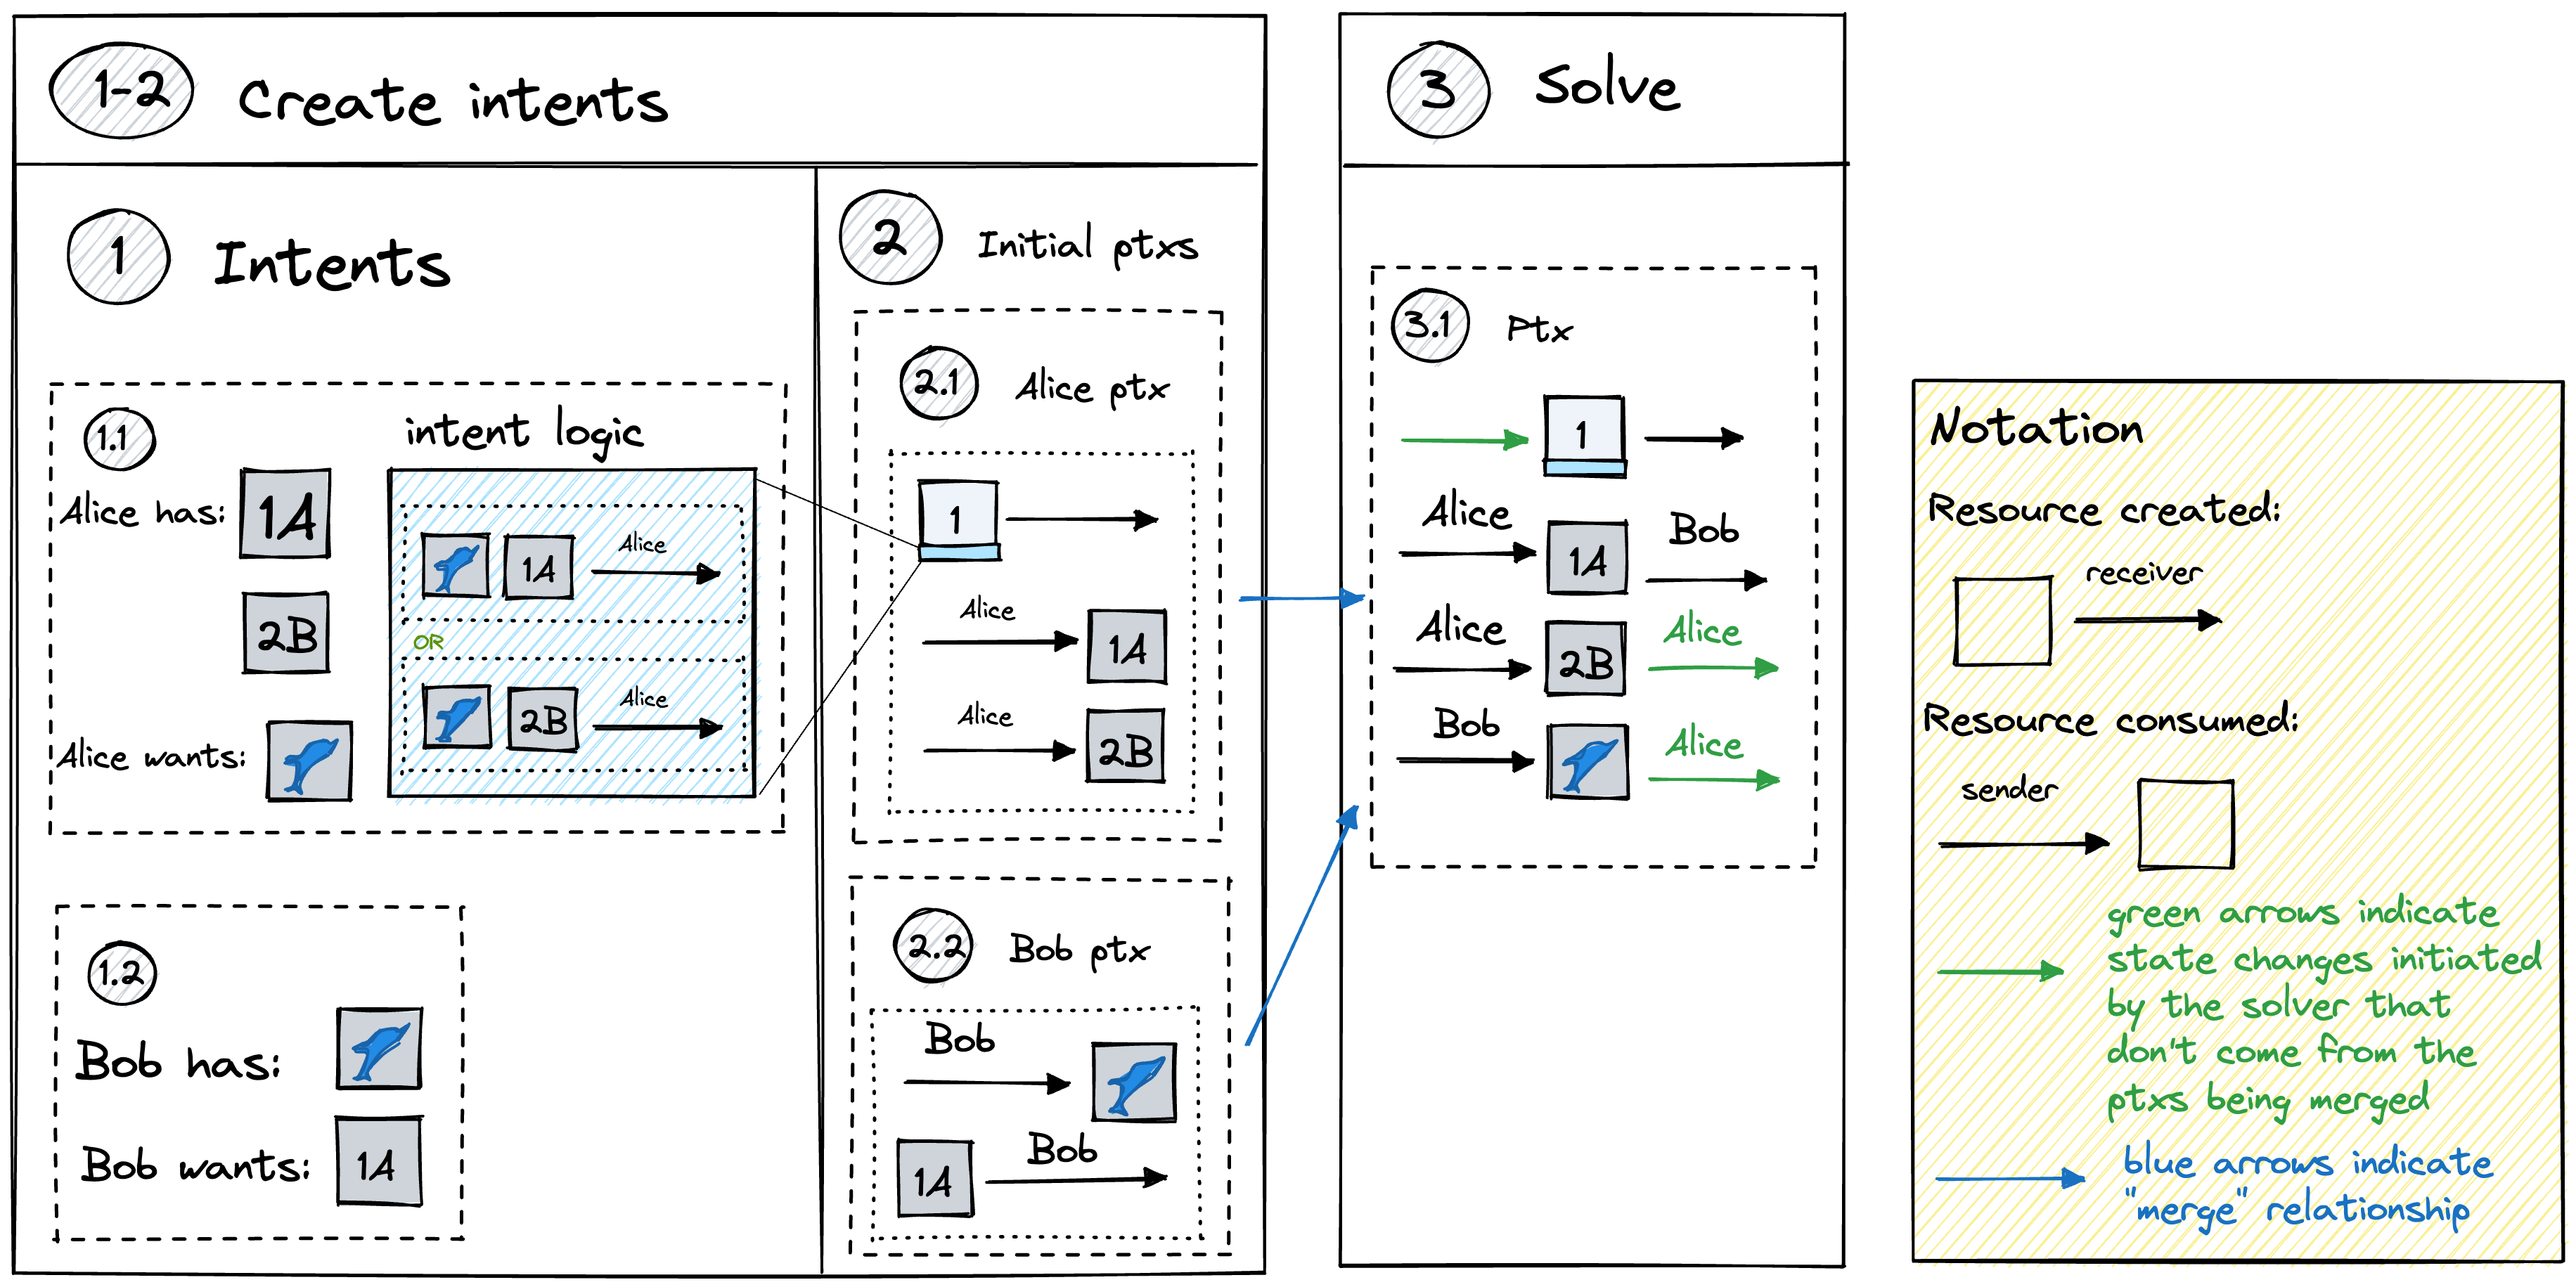
\includegraphics[width = \textwidth]{2party_rm_new.png}
\end{center}
\end{figure}

\begin{remark}
    For simplicity, in the examples in this paper, the set of compliance proofs for initial transactions (the transactions that were not composed of other transactions) is assumed to contain all the necessary compliance proofs, but the proofs themselves are not specified. Additionally, the delta proof aggregation function can take an arbitrary number of arguments. $AGG(X, Y, Z)$ in practice would be implemented as $AGG(AGG(X, Y), Z)$, similarly defined for any number of proofs.
\end{remark}

\textbf{Step 2:} create initial transactions

Alice creates a transaction $TX^A$ creating $R^A_I$, and consuming $R^A_{1A}$ and $R^A_{2B}$:
\begin{itemize}
    \item $rts= \{rt_{R^A_{1A}}, rt_{R^A_{2B}}\}$
    \item $cms = \{cm_{R^A_I}\}$
    \item $nfs = \{nf_{R^A_{1A}}, nf_{R^A_{2B}}\}$
    \item Proofs:
    \begin{itemize}
        \item $\Pi^A_{\Delta}$
        \item $\Pi^A_{compl}$
        \item $\Pi^A_{rl} = \{\pi^A_A, \pi^A_B, \pi^A_I\}$
    \end{itemize}
    \item $\Delta \mapsto \{I: 1, A: -1, B: -2\}$. For simplicity, represent $\Delta$ as a dictionary
    \item $extra = extra^A$
    \item $\Phi = \Phi^A$
\end{itemize}

Bob creates a transaction $TX^B$ creating $R^B_{1A}$ and consuming $R^B_{NFT}$:
\begin{itemize}
    \item $rts= \{rt_{R^B_{NFT}}\}$
    \item $cms = \{cm_{R^B_{1A}}\}$
    \item $nfs = \{nf_{R^B_{NFT}}\}$
     \item Proofs:
    \begin{itemize}
        \item $\Pi^B_{\Delta}$
        \item $\Pi^B_{compl}$
        \item $\Pi^B_{rl} = \{\pi^B_A, \pi^B_{NFT}\}$
    \end{itemize}
    \item $\Delta \mapsto \{NFT: -1, A: 1\}$
    \item $extra = extra^B$
    \item $\Phi = \Phi^B$
\end{itemize}

\textbf{Step 3:} solve

A solver $S$, having $TX^A$ and $TX^B$, creates a transaction $TX^S$:

\begin{itemize}
    \item $rts= \{rt_{R^A_{I}}\}$
    \item $cms = \{cm_{R^A_{2B}}, cm_{R^A_{NFT}}\}$
    \item $nfs = \{nf_{R^A_{I}}\}$
         \item Proofs:
    \begin{itemize}
        \item $\Pi^S_{\Delta}$
        \item $\Pi^S_{compl}$
        \item $\Pi^S_{rl} = \{\pi^S_B, \pi^S_{NFT}, \pi^S_I\}$
    \end{itemize}
    \item $\Delta \mapsto \{NFT: 1, B: 2, I: -1\}$
    \item $extra = extra^S$
    \item $\Phi = \Phi^S$
\end{itemize}

and composes all three transactions together, producing a balanced transaction $TX$:

\begin{itemize}
    \item $rts= \{rt_{R^A_{I}},
    rt_{R^A_{2B}},
    rt_{R^A_{1A}},  rt_{R^B_{NFT}}\}$
    \item $cms = cms^{A} \sqcup cms^B \sqcup cms^S = \{
    cm_{R^A_I}, cm_{R^A_{2B}}, cm_{R^A_{NFT}}, cm_{R^B_{1A}}\}$
    \item $nfs = nfs^A \sqcup nfs^B \sqcup nfs^S = \{nf_{R^A_{I}},
    nf_{R^A_{2B}},
    nf_{R^A_{1A}},  nf_{R^B_{NFT}}\}$
    \item Proofs:
    \begin{itemize}
        \item $\Pi_{\Delta} = AGG(\Pi^A_{\Delta}, \Pi^B_{\Delta}, \Pi^S_{\Delta})$
        \item $\Pi_{compl} = \Pi^A_{compl} \sqcup \Pi^B_{compl} \sqcup \Pi^S_{compl}$
        \item $\Pi_{rl} = \Pi^A_{rl} \sqcup \Pi^B_{rl} \sqcup \Pi^S_{rl}$
    \end{itemize}

    \item $\Delta \mapsto \{A: 0, B: 0, I: 0, NFT: 0\}$
    \item $extra = extra^A \cup extra^B \cup extra^S$
    \item $\Phi = G(\Phi^A, \Phi^B, \Phi^S)$
\end{itemize}

In practice, the step of creation of the transaction $TX_{S_1}$ can be merged with the composing step, but we separate the steps for clarity.

\section{Future directions}

This report contains the necessary information to build a resource machine that has the desired properties, but there are more properties we might want and more questions worth investigating. One such question would be whether resource logics should be able to see all resources in a transaction. This would allow us to perform \say{for all} checks — for example, a resource logic might want to enforce a non-inclusion of resources of a certain type in this transaction. However, enforcing such a feature is a non-trivial task, and it is not clear if it is as beneficial as it seems: for example, if there is a valid way to escape such checks (e.g., by wrapping a resource in another resource kind), it won’t be helpful to have a mechanism for checking. 

%\section{Concluding remarks}
%\section{Acknowledgements}
\nocite{*}
\bibliography{ref.bib}

\appendix
\section{Three-party NFT exchange cycle}
Another example is a three-party exchange cycle. Each party uses ephemeral resource logics to express their intents.
\hfill\break
\hfill\break
\textbf{Step 1:} specify intents

\begin{itemize}
    \item \textbf{Alice's intent:} Alice wants to exchange her star NFT resource $R^A_{star}$ for a blue dolphin NFT resource $R_{dolphin}$
    \item \textbf{Bob's intent:} Bob wants to exchange his blue dolphin NFT $R^B_{dolphin}$ for a tree NFT resource $R_{tree}$
    \item \textbf{Charlie's intent:} Charlie wants to exchange his tree NFT $R^C_{tree}$ for a star NFT resource $R_{star}$
\end{itemize}

\begin{center}
    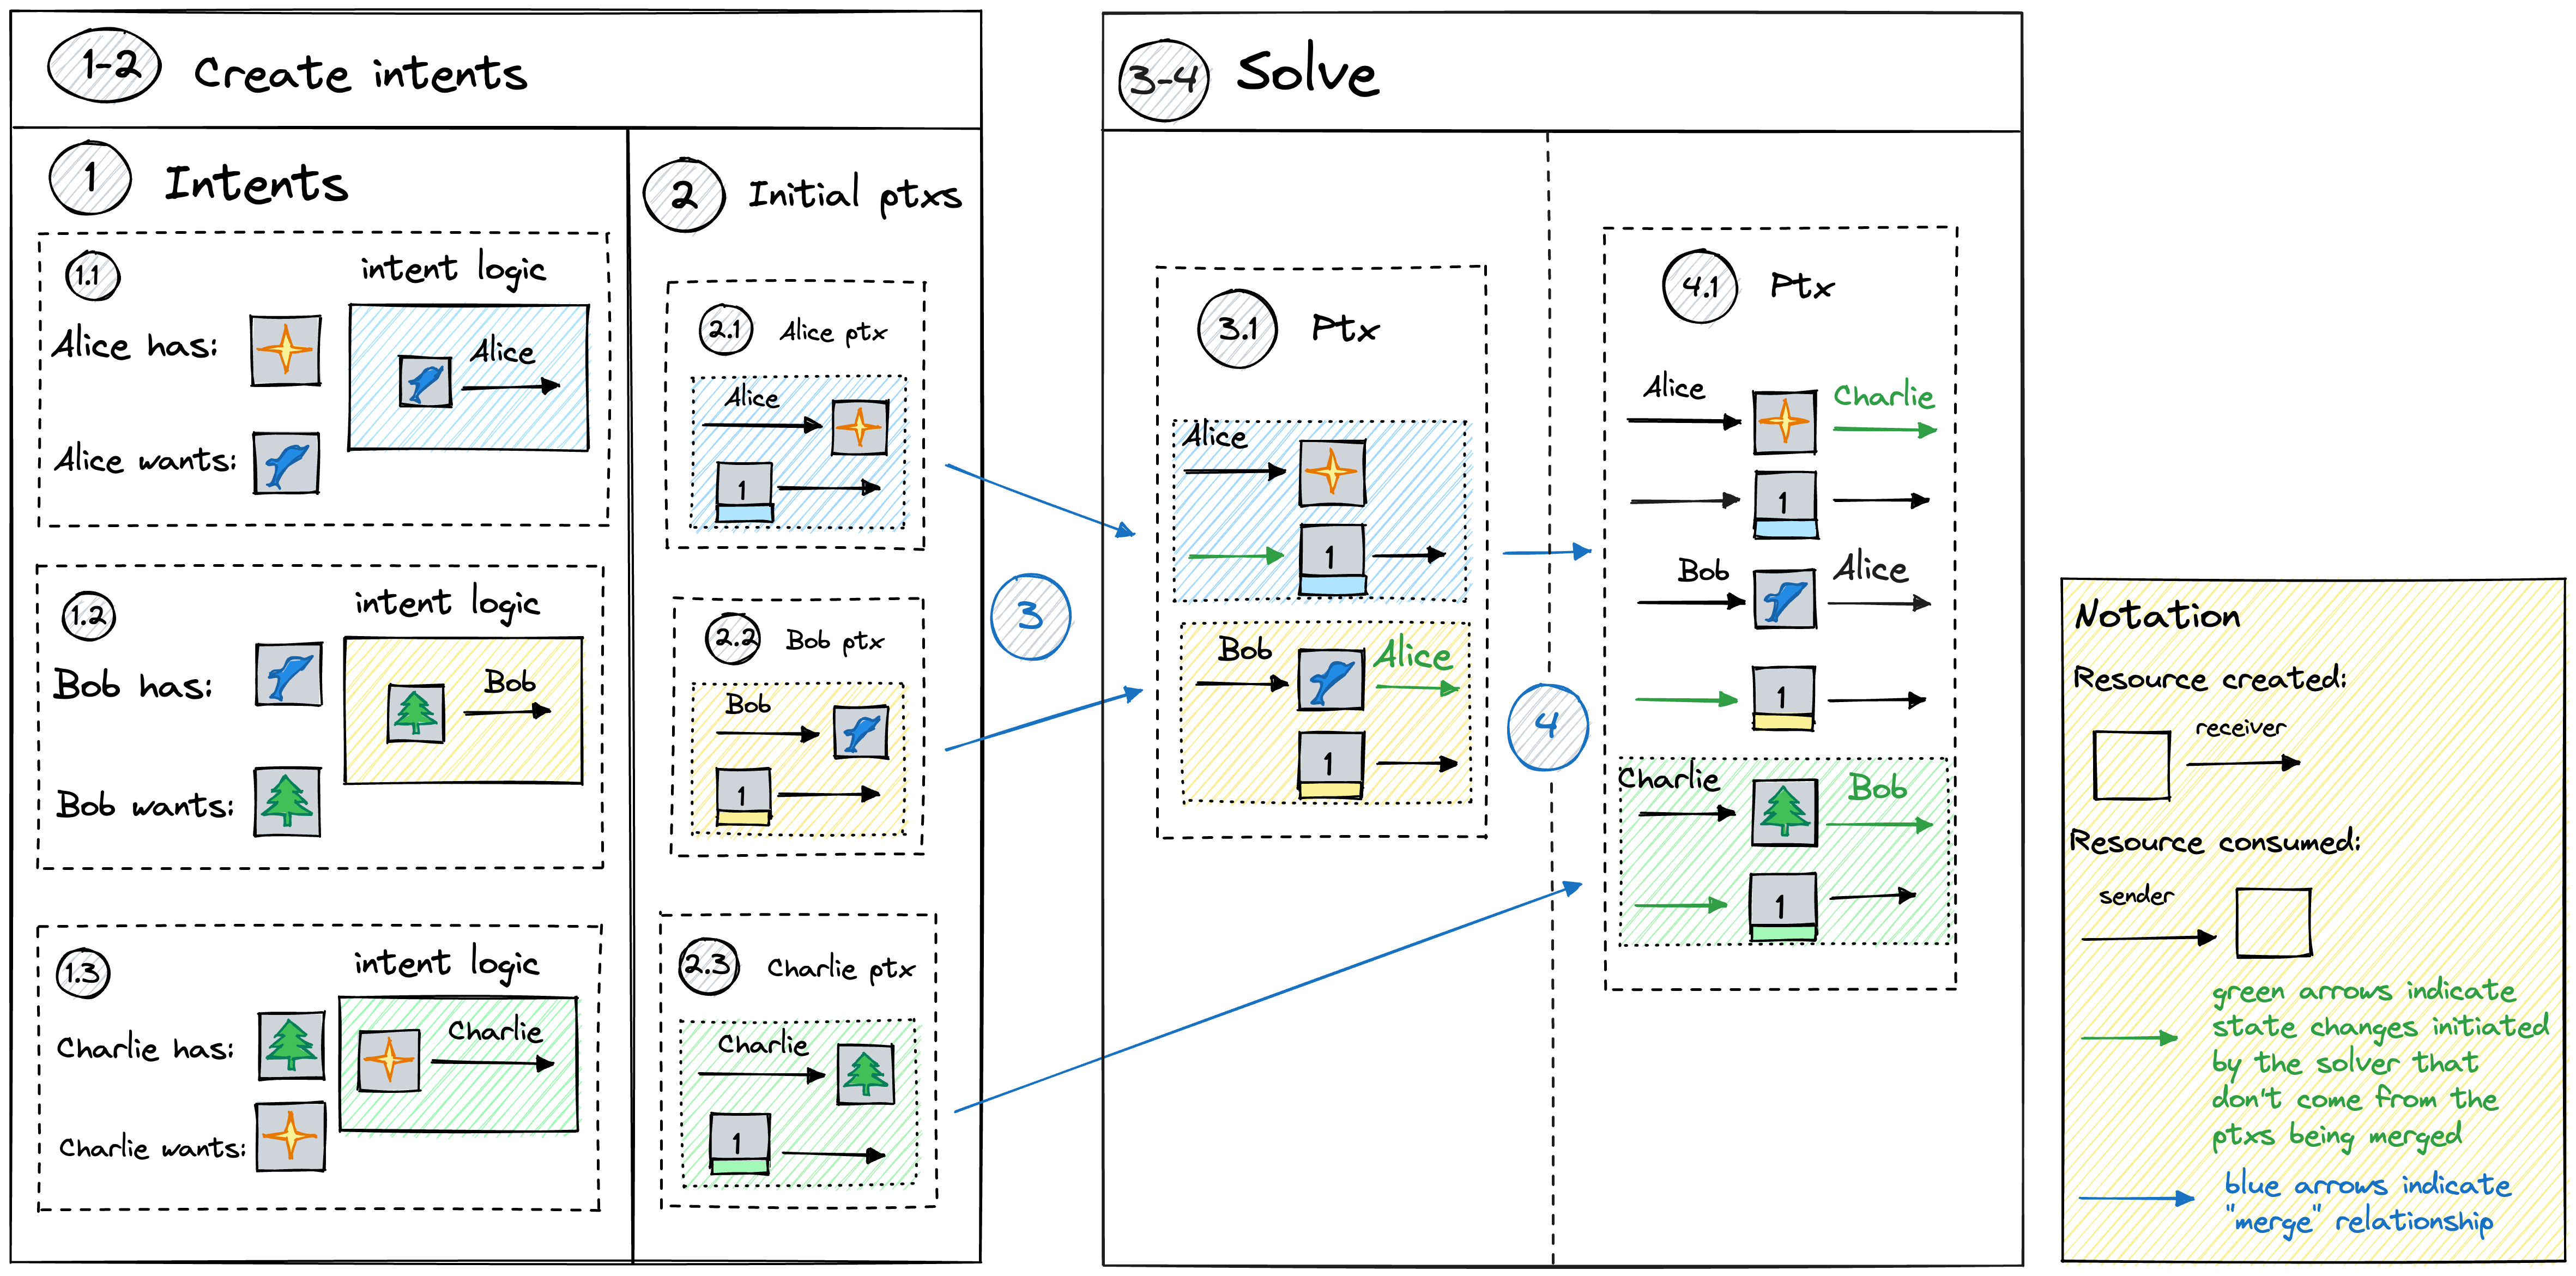
\includegraphics[width = \textwidth]{3party_rm_new.png}
\end{center}

\textbf{Step 2:} create initial transactions

Alice's initial transaction:
\begin{itemize}
    \item $rts= \{rt_{R^A_{star}}\}$
    \item $cms = \{cm_{R^A_{I^{A}}}\}$
    \item $nfs = \{nf_{R^A_{star}}\}$
    \item Proofs:
    \begin{itemize}
        \item $\Pi^A_{\Delta}$
        \item $\Pi^A_{compl}$
        \item $\Pi^A_{rl} = \{\pi^A_{star}, \pi^A_I\}$
    \end{itemize}
    \item $\Delta \mapsto \{I^{A}: 1, star: -1, \}$ – for simplicity, represent $\Delta$ as a dictionary
    \item $extra = extra^A$
    \item $\Phi = \Phi^A$
\end{itemize}

Bob's initial transaction:
\begin{itemize}
    \item $rts = \{rt_{R^B_{dolphin}}\}$
    \item $cms = \{cm_{R^B_{I^{B}}}\}$
    \item $nfs = \{nf_{R^B_{doplhin}}\}$
    \item Proofs:
    \begin{itemize}
        \item $\Pi^B_{\Delta}$
        \item $\Pi^B_{compl}$
        \item $\Pi^B_{rl} = \{\pi^B_{dolphin}, \pi^B_I\}$
    \end{itemize}
    \item $\Delta \mapsto \{I^{B}: 1, dolphin: -1 \}$
    \item $extra = extra^B$
    \item $\Phi = \Phi^B$
\end{itemize}

Charlie's initial transaction:
\begin{itemize}
    \item $rts = \{rt_{R^C_{tree}}\}$
    \item $cms = \{cm_{R^C_{I^{C}}}\}$
    \item $nfs = \{nf_{R^C_{tree}}\}$
    \item Proofs:
    \begin{itemize}
        \item $\Pi^C_{\Delta}$
        \item $\Pi^C_{compl}$
        \item $\Pi^C_{rl} = \{\pi^C_{tree}, \pi^C_I\}$
    \end{itemize}
    \item $\Delta \mapsto \{I^{C}: 1, tree: -1, \}$
    \item $extra = extra^C$
    \item $\Phi = \Phi^C$
\end{itemize}

\textbf{Step 3:} solve

A solver $S_1$, seeing $TX^A$ and $TX^B$, creates a transaction $TX^{S_1}$ (on the diagram: $TX_{3.1}$, green arrows):

\begin{itemize}
    \item $rts = \{rt_{R^A_{I^{A}}}\}$
    \item $cms = \{cm_{R^A_{dolphin}}\}$
    \item $nfs = \{nf_{R^A_{I^{A}}}\}$
        \item Proofs:
    \begin{itemize}
        \item $\Pi^{S_1}_{\Delta}$
        \item $\Pi^{S_1}_{compl}$
        \item $\Pi^{S_1}_{rl} = \{\pi^{S_1}_{dolphin}, \pi^{S_1}_{I_A}\}$
    \end{itemize}
    \item $\Delta \mapsto \{dolphin: 1, I^{A}: -1\}$
    \item $extra = extra^{S_1}$
    \item $\Phi = \Phi^{S_1}$
\end{itemize}

and composes all three transactions together, producing a transaction $TX_{3.1}$:

\begin{itemize}
    \item $rts = \{rt_{R^A_{star}}, rt_{R^B_{dolphin}}, rt_{R^A_{I^{A}}}\}$
    \item $cms = cms^{A} \sqcup cms^B \sqcup cms^{S_1} =\{
    cm_{R^A_{I^{A}}}, cm_{R^B_{I^{B}}}, cm_{R^A_{dolphin}}\}$
    \item $nfs = nfs^A \sqcup nfs^B \sqcup nfs^{S_1} = \{nf_{R^A_{star}}, nf_{R^B_{dolphin}}, nf_{R^A_{I^{A}}}\}$
        \item Proofs:
    \begin{itemize}
        \item $\Pi^{3.1}_{\Delta} = AGG(\Pi^A_{\Delta}, \Pi^B_{\Delta}, \Pi^{S_1}_{\Delta})$
        \item $\Pi^{3.1}_{compl} = \Pi^A_{compl} \sqcup \Pi^B_{compl} \sqcup \Pi^{S_1}_{compl}$
        \item $\Pi^{3.1}_{rl} = \Pi^A_{rl} \sqcup \Pi^B_{rl} \sqcup \Pi^{S_1}_{rl}$
    \end{itemize}
    \item $\Delta \mapsto \{I^{A}: 0, I^{B}: 1, star: -1, dolphin: 0\}$
    \item $extra = extra^A \cup extra^B \cup extra^{S_1}$
    \item $\Phi = G(\Phi^A, \Phi^B, \Phi^{S_1})$
\end{itemize}

\textbf{Step 4:} continue solving

Seeing $TX^C$ and $TX_{3.1}$, a solver $S_2$ creates a transaction $TX_{S_2}$ (on the diagram: $TX_{4.1}$, green arrows):

\begin{itemize}
    \item $rts = \{rt_{R^C_{I^{C}}}, rt_{R^B_{I^{B}}}\}$
    \item $cms = \{
    cm_{R^C_{star}}, cm_{R^B_{tree}}\}$
    \item $nfs = \{nf_{R^C_{I^{C}}}, nf_{R^B_{I^{B}}}\}$
    \item Proofs:
    \begin{itemize}
        \item $\Pi^{S_2}_{\Delta}$
        \item $\Pi^{S_2}_{compl}$
        \item $\Pi^{S_2}_{rl} = \{\pi^{S_2}_{star}, \pi^{S_2}_{I_C}\, \pi^{S_2}_{tree}, \pi^{S_2}_{I_B}\}$
    \end{itemize}
    \item $\Delta \mapsto \{I^{C}: -1, I^{B}: -1, star: 1, tree: 1\}$
    \item $extra = extra^{S_2}$
    \item $\Phi = \Phi^{S_2}$
\end{itemize}

and composes all three into a balanced transaction $TX_{4.1}$:

\begin{itemize}
    \item $rts = \{rt_{R^A_{star}}, rt_{R^B_{dolphin}}, rt_{R^C_{tree}}, rt_{R^A_{I^{A}}}, rt_{R^B_{I^{B}}}, rt_{R^C_{I^{C}}}\}$
    \item $cms = cms^{TX^{3.1}} \sqcup cms^{S_2} =\{cm_{R^A_{dolphin}}, cm_{R^B_{tree}}, cm_{R^C_{star}}, cm_{R^A_{I^{A}}}, cm_{R^B_{I^{B}}}, cm_{R^C_{I^{C}}}\}$
    \item $nfs = nfs^{TX^{3.1}} \sqcup nfs^{S_2} = \{nf_{R^A_{star}}, nf_{R^B_{dolphin}}, nf_{R^C_{tree}}, nf_{R^A_{I^{A}}}, nf_{R^B_{I^{B}}}, nf_{R^C_{I^{C}}}\}$
    \item Proofs:
    \begin{itemize}
        \item $\Pi^{4.1}_{\Delta} = AGG(\Pi^{3.1}_{\Delta}, \Pi^{C}_{\Delta}, \Pi^{S_2}_{\Delta})$
        \item $\Pi^{4.1}_{compl} = \Pi^C_{compl} \sqcup \Pi^{3.1}_{compl} \sqcup \Pi^{S_2}_{compl}$
        \item $\Pi^{4.1}_{rl} = \Pi^C_{rl} \sqcup \Pi^{3.1}_{rl} \sqcup \Pi^{S_2}_{rl}$
    \end{itemize}
    \item $\Delta \mapsto \{I^{A}: 0, I^{B}: 0, I^{C}: 0, star: 0, dolphin: 0, tree: 0\}$
    \item $extra = extra^A \cup extra^B \cup extra^C \cup extra^{S_1} \cup extra^{S_2}$
    \item $\Phi = G(\Phi^A, \Phi^B, \Phi^{S_1}, \Phi^C, \Phi^{S_2})$
\end{itemize}

In practice, the step of creation of the transactions $TX_{S_1}$ and $TX_{S_2}$ can be merged with the composing step, but we separate the steps for clarity.

\end{document}
